\documentclass[fontsize=12pt]{scrartcl}

\newcommand{\grad}{\ensuremath{^{\circ}} }
\renewcommand{\strut}{\vrule width 0pt height5mm depth2mm}

\usepackage[utf8]{inputenc}
\usepackage[final]{pdfpages}
% obere Seitenränder gestalten können
\usepackage{fancyhdr}
\usepackage{moreverb}
% Graphiken als jpg, png etc. einbinden können
\usepackage{graphicx}
%\usepackage{stmaryrd}
% Floats Objekte mit [H] festsetzen
\usepackage{float}
% setzt URLs schön mit \url{http://bla.laber.com/~mypage}
\usepackage{url}
% Externe PDF's einbinden können
\usepackage{pdflscape}
% Verweise innerhalb des Dokuments schick mit " ... auf Seite ... "
% automatisch versehen. Dazu \vref{labelname} benutzen
\usepackage[ngerman]{varioref}
\usepackage[ngerman]{babel}
\usepackage{ngerman}
% Bibliographie
\usepackage{bibgerm}
% Tabellen
\usepackage{tabularx}
\usepackage{supertabular}
\usepackage[colorlinks=true, pdfstartview=FitV, linkcolor=blue,
            citecolor=blue, urlcolor=blue, hyperfigures=true,
            pdftex=true]{hyperref}
\usepackage{bookmark}
\usepackage[a4paper]{geometry}

% Damit Latex nicht zu lange Zeilen produziert:
\sloppy
%Uneinheitlicher unterer Seitenrand:
%\raggedbottom

% Kein Erstzeileneinzug beim Absatzanfang
% Sieht aber nur gut aus, wenn man zwischen Absätzen viel Platz einbaut
\setlength{\parindent}{0ex}

% Abstand zwischen zwei Absätzen
\setlength{\parskip}{1ex}

% Lustige Header auf den Seiten
  \pagestyle{fancy}
 \setlength{\headheight}{70.55003pt}
  \fancyhead{}
  \fancyhead[LO,RE]{Benutzerhandbuch}
  \fancyhead[LE,RO]{Seite \thepage\\\slshape \leftmark\\\slshape \rightmark}

%
% Und jetzt geht das Dokument los....
%

\begin{document}

% Start Titelseite
  \thispagestyle{empty}
  \newgeometry{hmarginratio=1:1}
  \vspace{3cm}
  \begin{minipage}[H]{\textwidth}
  \begin{center}
  \vspace{1cm}
  \bf
  {\Large Benutzerhandbuch}\\
  der Stundenplansoftware \\
  der Gruppe\\
    \begin{figure}[H]
    \centering
    
\includegraphics[width=0.15\textwidth]{../WOYM.png}
    \end{figure}
  \vfill
  \end{center}
  \end{minipage}
  \vfill
  \begin{minipage}[H]{\textwidth}
  \begin{center}
  \sf
  \begin{tabular}{l}
  Tim Hansen \\\
  Adrian Lück \\
  Jurij Schmidt\\
  \end{tabular}
  \end{center}
  \end{minipage}
\restoregeometry
% Ende Titelseit

% Start Leerseite
\cleardoubleemptypage

%Start Inhaltsverzeichnis
\newpage

  \thispagestyle{fancy}
  \fancyhead{}
  \fancyhead[LO,RE]{Benutzerhandbuch}
  \fancyhead[LE,RO]{Seite \thepage\\\slshape \leftmark~}
  \fancyfoot{}
  \renewcommand{\headrulewidth}{0.4pt}
  \tableofcontents

\newpage
  \fancyhead[LE,RO]	{Seite \thepage\\ \slshape \leftmark \\ \slshape \rightmark}

\section{Systemanforderungen}
\begin{itemize}
\item Java 7 oder neuer
\item ein aktueller Webbrowser
\end{itemize}

\section{Installation und Inbetriebnahme}

Entpacken Sie die ausgelieferte ZIP-Datei in das von Ihnen für die Software gewünschte Arbeitsverzeichnis. 

\subsection{Windows-Betriebssysteme}
Unter Windows können Sie die Datei \textit{start.bat} verwenden, um die Software zu starten. Wenn Sie die Datei anklicken öffnet sich die Windows-Konsole und der für die Software benötigte Server startet. Gleichzeitig öffnet sich Ihr Browser-Fenster und lädt die Startseite der Software, sobald der Server komplett hochgefahren ist. Schließen Sie die Windows-Konsole nur, wenn Sie die Software beenden wollen. Ansonsten muss Sie für den Betrieb der Software geöffnet bleiben.\\
Wenn Sie wünschen, die Software vom Desktop aus starten zu können, legen Sie eine Verknüpfung zu der Datei \textit{start.bat} an.\\
So lange die Software in der Konsole läuft, können Sie die Startseite unter \url{http://localhost:8080/timetable} erreichen.\\

Sollte ein Start mittels der \textit{start.bat} nicht funktionieren, müssen Sie ggf. Ihre Java PATH-Systemvariable setzen.

\subsection{Linux- / Mac-Betriebssysteme}
Für Linux- oder Mac-Betriebssysteme liegt das Skript \textit{startstop.sh} bei. Dieses kann über das Terminal mit den Parametern \textit{start}, \textit{stop}, \textit{restart} bzw. \textit{reload} oder \textit{status} ausgeführt werden um die Software zu starten, stoppen, neu zu starten oder den Status abzufragen. Die Software wird durch Schließen der Konsole nicht automatisch beendet.

\section{Bedienung der Software}

\subsection{Allgemeine Informationen}

Sie können nahezu alle Aktionen, die sie ausgeführt haben rückgängig machen oder das Rückgängigmachen wiederholen. Die einzige Ausnahme bildet das Ändern der Systemeinstellungen. Dies lässt sich nur manuell rückgängig machen und alle Aktivitäten, die dabei möglicherweise gelöscht wurden, lassen sich nicht wiederherstellen ohne ein Backup eines vorherigen Zeitpunktes zu laden.\\

Die Software ist grundsätzlich in zwei Seiten, die Einrichtungs- und die Planungsseite eingeteilt. Auf beiden Seiten werden Sie oben eine angepinnte Toolbar finden, welche Ihnen das Rückgängigmachen und Wiederherstellen von bis zu zehn Aktionen und das Wechseln auf die jeweils andere Seite erlaubt. Beispielhaft ist hier die Toolbar der Einrichtungsseite dargestellt.

\begin{figure}[H]
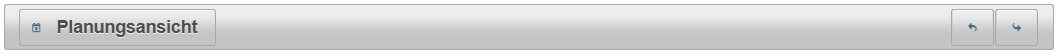
\includegraphics[width=\textwidth]{images/bar.png}
\caption{Toolbar der Einstellungsseite}
\end{figure}

\subsection{Die Einrichtungsseite}
Die Einrichtungsseite dient der Vorbereitung zur Planung. Sie legen dort Standorte und Räume, Unterrichtsinhalte, Schulklassen, Personen des Personals und Klassenteams an und verwalten ihre Systemeinstellungen und Backups. Es wird empfohlen zunächst die Systemeinstellungen an Ihre Bedürfnisse anzupassen und anschließend die Objekte nach der Reihenfolge des Navigationsmenüs von oben nach unten hinzuzufügen.
\begin{figure}[H]
\centering
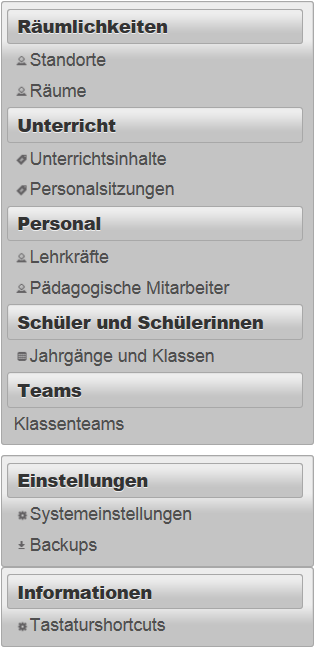
\includegraphics[width=0.3\textwidth]{images/navigationMenu.png}
\caption{Navigationsmenü auf der Einstellungsseite}
\end{figure}

Da für das Hinzufügen, Bearbeiten und Löschen aller Objekte dieselbe Mechanik verwendet wird, wird dies im Folgenden lediglich am Beispiel einer Lehrkraft erläutert.

\subsubsection{Systemeinstellungen}
In den Systemeinstellungen können Sie verschiedene Parameter der Software selbst festlegen.\\

Zunächst einmal haben Sie in den Systemeinstellungen die Möglichkeit, alle Aktivitäten zu löschen, falls Sie eine komplett neue Planung beginnen möchten. Diesen Schritt können Sie rückgängig machen. 

\begin{figure}[H]
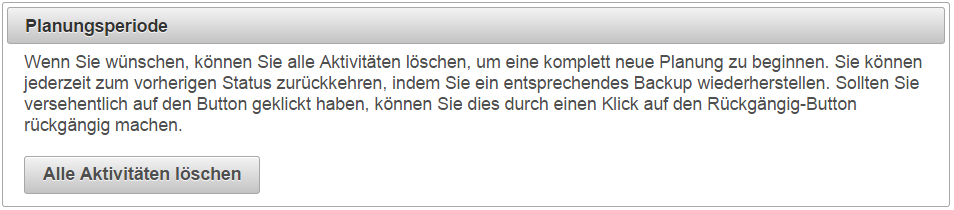
\includegraphics[width=\textwidth]{images/systemSettings1.png}
\caption{Einstellungsseite: Alle Aktivitäten löschen}
\end{figure}

Des Weiteren können Sie die allgemeinen Einstellungen der Software verändern. So haben Sie etwa die Möglichkeit die zu verplanenden Wochentage, Start- und Endzeit eines Wochentags und die Größe des Zeitrasters des Stundenplans festzulegen. Außerdem können Sie angeben, wie die zeitliche Abrechnung des Personals erfolgen soll, welche Bezeichner sie für Schulklassen wünschen und wie lang die typische Dauer einer Aktivität sein soll. Sie können hier zudem alle Dialoge zurücksetzen, so dass diese erneut beim Löschen angezeigt werden. \\

\fbox{\parbox{\textwidth}{\textbf{Achtung!} Wenn Sie die zu verplanenden Wochentage oder die Start- und Endzeit eines Wochentages ändern, werden alle Aktivitäten gelöscht, die an nicht mehr gewählten Wochentagen und außerhalb der neuen Start- und Endzeit liegen. Dies lässt sich \textbf{nicht} über den Rückgängig-Button rückgängig machen. Stattdessen müssten Sie ein Backup eines Zeitpunktes laden, wo sich die Aktivitäten noch im System befinden.}}

\begin{figure}[H]
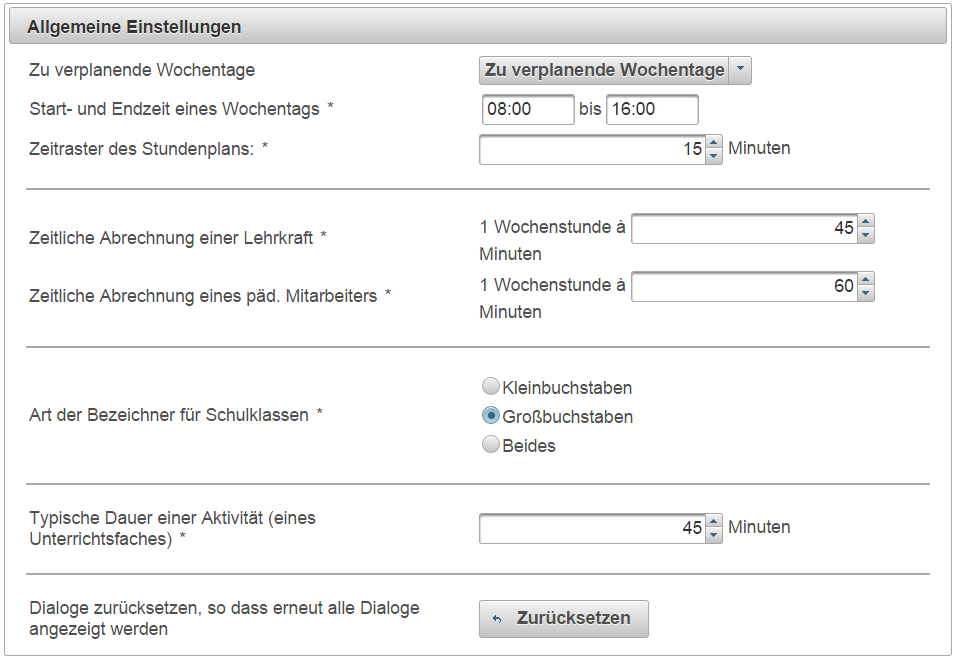
\includegraphics[width=\textwidth]{images/systemSettings2.png}
\caption{Allgemeine Einstellungen}
\end{figure}


Schließlich können Sie auf der Einstellungsseite auch noch das Intervall für automatische Backups festlegen. Hier können Sie wählen, dass Sie keine automatischen Backups, Backups in einem gewissen Minutentakt oder Backups in einem gewissen Tagestakt zu einer bestimmten Uhrzeit wünschen. Wenn Sie letztere Option wählen und die Software zu dem eigentlichen Backup-Zeitpunkt nicht gestartet ist, wird beim nächsten Programmstart nachträglich ein Backup ausgeführt.

\fbox{\parbox{\textwidth}{\textbf{Achtung!} Beachten Sie, dass Backups nicht automatisch gelöscht werden! Für weitere Informationen bezüglich der Backups, lesen Sie das folgende Kapitel.}}
 
\begin{figure}[H]
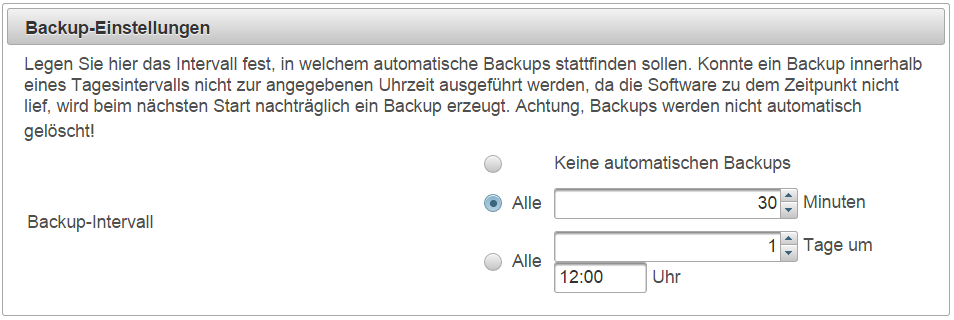
\includegraphics[width=\textwidth]{images/systemSettings3.png}
\caption{Backup-Einstellungen}
\end{figure}

\subsubsection{Anlegen und Wiederherstellen von Backups}

In dieser Software entspricht ein Backup im Grunde einem Speicherstand des System zu einem gewissen Zeitpunkt. In einem Backup ist nicht nur der Datenbankzustand, sondern auch die Systemeinstellungen des Zeitpunktes, an welchem das Backup erstellt wurde, vorhanden. Wie aus dem vorherigen Kapitel hervorging, ist die Software in der Lage Backups automatisch im Hintergrund zu erzeugen. Zusätzlich oder wenn Sie die automatischen Backups ausgeschaltet haben, können Sie aber auch manuell Backups erzeugen. \\
Sie haben die Auswahl, ob ein Backup einen automatisch aus dem aktuellen Datum und der Uhrzeit generierten Namen tragen soll oder ob sie es selbst benennen möchten.\\
Die Backups werden in Ihrem Benutzer-Ordner, wo sich auch der aktuelle genutzte Datenbankzustand befindet, gespeichert. Unter Windows ist der Pfad zum Backup-Ordner \textit{C:\textbackslash{}Users\textbackslash{}Username\textbackslash{}WOYM} unter Linux/Mac-OS \textit{/home/username/WOYM}. Dort werden die Backups als ZIP-Dateien abgelegt.\\
Die Backups werden auf der Backupverwaltung-Seite absteigend nach Erstellungsdatum sortiert.\\
Backups werden nicht automatisch gelöscht, dies müssen sie manuell übernehmen.

\begin{figure}[H]
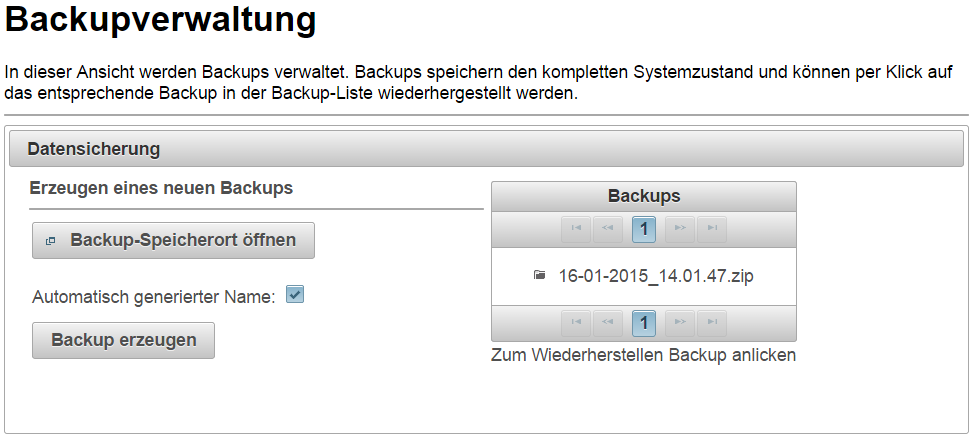
\includegraphics[width=\textwidth]{images/backupManagement.png}
\caption{Backupverwaltung}
\end{figure}

\subsubsection{Hinzufügen eines Objektes am Beispiel einer Lehrkraft}
\begin{enumerate}
\item Klicken Sie im Menü auf der linken Seite auf den Eintrag "`Lehrkräfte"'.
\item Sie sehen nun eine Tabelle, in welcher alle vorhandenen Lehrkräfte angezeigt werden. Klicken Sie auf den "`Hinzufügen"'-Button oben rechts.
\item Das folgende Dialogfenster öffnet sich: \medskip\\
	\begin{minipage}[t]{\linewidth}
            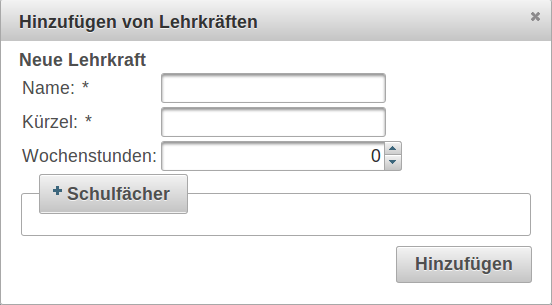
\includegraphics[width=.8\linewidth]{images/addTeacherDialog.png}
    \medskip\\
    Die mit * gekennzeichneten Angaben sind Pflichtangaben. Der Eintrag "`Schulfächer"' ist aufklappbar. Aufklappbare Angaben sind immer optional.
    \end{minipage}
\clearpage
\item Machen Sie alle gewünschten Angaben und klicken Sie anschließend auf "`Hinzufügen"'. Sie werden darüber informiert, wenn das Hinzufügen erfolgreich war: \medskip\\
	\begin{minipage}[t]{\linewidth}
            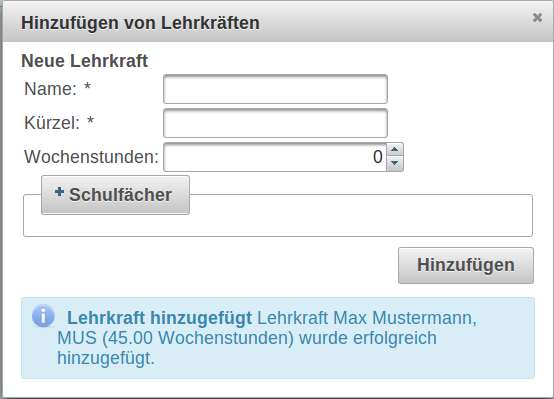
\includegraphics[width=.8\linewidth]{images/addedTeacher.png}
    \medskip\\
    Das Dialogfenster bleibt geöffnet, um das Hinzufügen weiterer Lehrkräfte zu erlauben. Wenn Sie keine weitere Lehrkraft hinzufügen möchten, klicken Sie auf das X in der oberen rechten Ecke des Dialogs.
    \end{minipage}
\end{enumerate}

\subsubsection{Aktualisieren eines Objektes am Beispiel einer Lehrkraft}

\begin{enumerate}
\item Führen Sie einen Rechtsklick auf die zu bearbeitende Lehrkraft aus und wählen sie "`Bearbeiten"': \medskip\\
	\begin{minipage}[t]{\linewidth}
            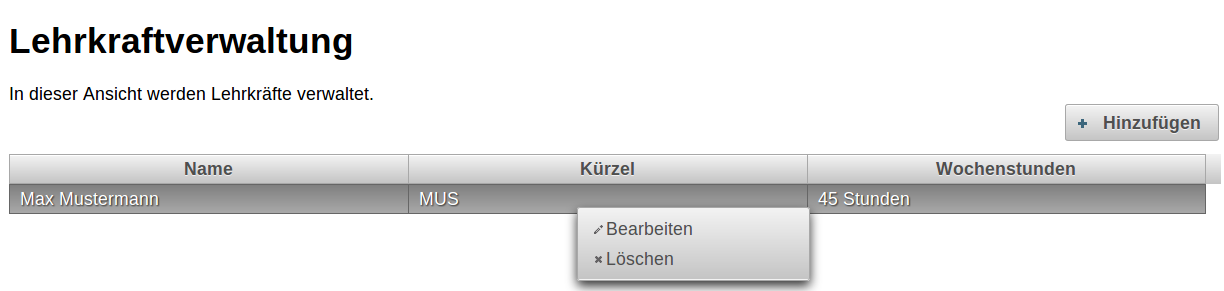
\includegraphics[width=1\linewidth]{images/editTeacher.png}
    \end{minipage}
\item Im dem sich öffnenden Dialogfenster sind alle Angaben der gewählten Lehrkraft eingetragen: \medskip\\
	\begin{minipage}[t]{\linewidth}
            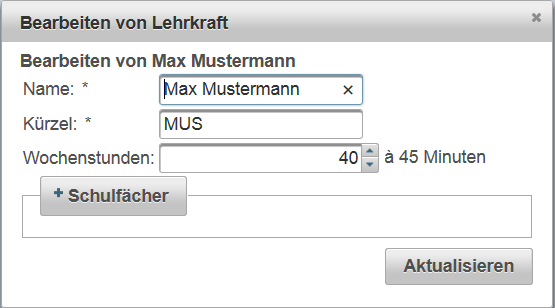
\includegraphics[width=.8\linewidth]{images/editTeacherDialog.png}
    \medskip\\ Passen Sie die Angaben nach Belieben an.
    \end{minipage}
\item Klicken Sie auf "`Aktualisieren"'. Bei Erfolg schließt sich das Dialogfenster und Sie werden über die erfolgreiche Aktualisierung informiert. 
\end{enumerate}

\subsubsection{Löschen eines Objektes am Beispiel einer Lehrkraft}
\begin{enumerate}
\item Führen Sie einen Rechtsklick auf die zu bearbeitende Lehrkraft aus und wählen sie "`Löschen"': \medskip\\
	\begin{minipage}[t]{\linewidth}
            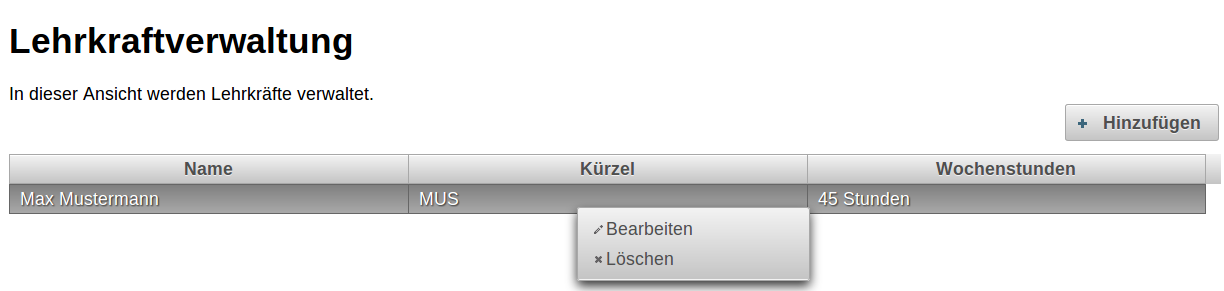
\includegraphics[width=1\linewidth]{images/editTeacher.png}
    \end{minipage}
\item Es öffnet sich ein Dialogfenster, welches Sie über die Folgen des Löschens aufklärt. Da Sie alle Aktionen rückgängig machen können, haben Sie die Option, das Dialogfenster zukünftig nicht mehr anzeigen zu lassen. \medskip\\
	\begin{minipage}[t]{\linewidth}
            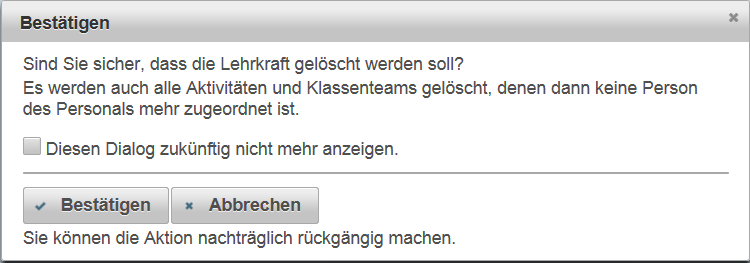
\includegraphics[width=.8\linewidth]{images/confirmDialog.png}
    \end{minipage} 
\end{enumerate}

\subsection{Die Planungsseite}
Beim Start der Software wird Ihnen immer die Planungsseite anzeigt. Auf dieser Seite können Sie die Stundenpläne des Personals und der Klassen und Raumbelegungspläne verwalten. Über den Button "`Alternative Anzeigen"' können Sie außerdem den Lehrkrafteinsatz- und den Wochentagplan einsehen.

\begin{figure}[H]
\centering
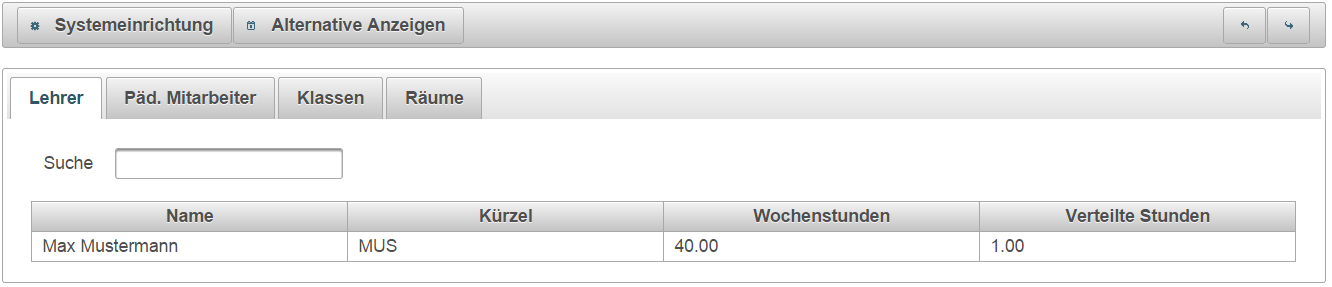
\includegraphics[width=\textwidth]{images/planningPage.png}
\end{figure}

Um einen Stundenplan anzuzeigen, klicken Sie die gewünschte Person des Personals, die Schulklasse oder den Raum an.

\begin{figure}[H]
\centering
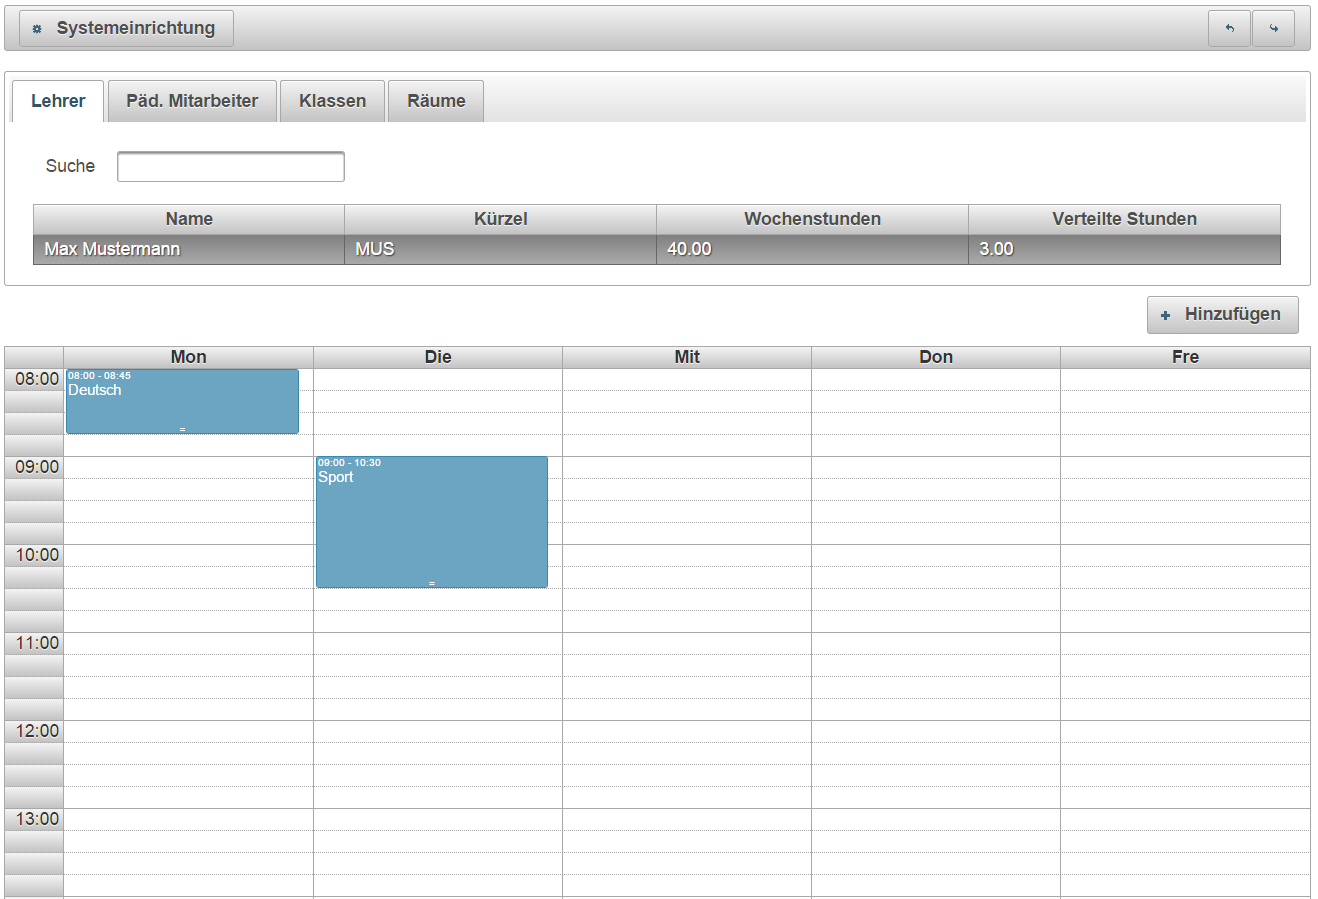
\includegraphics[width=\textwidth]{images/planningPage2.png}
\end{figure}

\subsubsection{Hinzufügen einer Aktivität}
Um den Dialog für das Hinzufügen einer Aktivität zu öffnen, stehen Ihnen zwei Möglichkeiten bereit: 
\begin{itemize}
\item Verwenden Sie den "`Hinzufügen"'-Button oben rechts über dem Plan.
\item Klicken Sie auf gewünschten Starttermin der Aktivität (Tag und Uhrzeit). Dies ist der deutliche effizientere Weg, da Tag und Zeiten nicht mehr manuell eingetragen werden müssen.
\end{itemize}

\begin{enumerate}
\item Wählen Sie im geöffneten Dialog zunächst aus, was sie dem Plan hinzufügen möchten: \medskip\\
	\begin{minipage}[t]{\linewidth}
            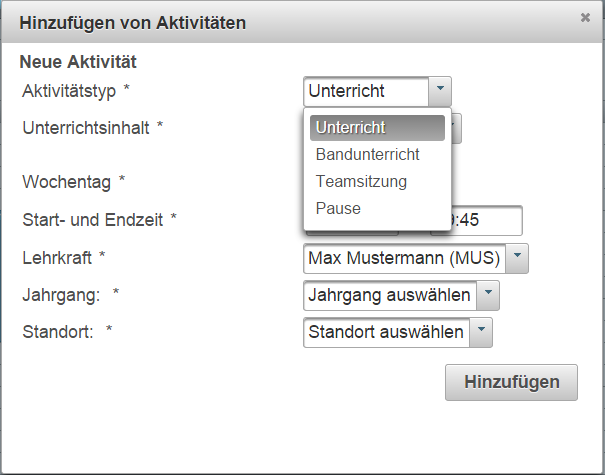
\includegraphics[width=.8\linewidth]{images/addActivity.png}
    \end{minipage} 
    \medskip
    Je nach Auswahl werden andere Eingabefelder angezeigt.
    \clearpage
\item Machen Sie alle weiteren Angaben.\medskip\\
	\begin{minipage}[t]{\linewidth}
            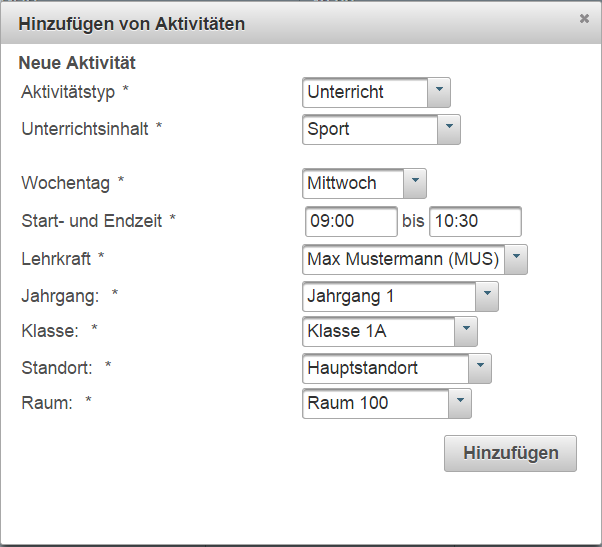
\includegraphics[width=.8\linewidth]{images/addActivity2.png}
    \end{minipage} 
    \medskip\\
    Die Endzeit im Hinzufügen-Dialog für Unterricht und Personalsitzungen wird entsprechend der typischen Dauer des ausgewählten Unterrichtsinhaltes / Sitzungstyps automatisch gesetzt. \\
    Bei Personalsitzungen wird außerdem automatisch der für den ausgewählten Sitzungstyp angegeben Raum gewählt. \\
    Beim Unterricht wird der Raum des Unterrichtsinhalts nur dann gewählt, wenn es sich um einen Raum handelt, der nicht die Funktion "`Standardraum"' besitzt. Ansonsten wird er Klassenraum der Klasse gesetzt.\\
    Alle diese automatisch gesetzten Werte können natürlich nachträglich noch verändert werden.
\item Klicken Sie anschließend auf Hinzufügen. Wenn das Hinzufügen erfolgreich ist, wird der Dialog geschlossen.
\end{enumerate}

\subsubsection{Nähere Informationen zu Aktivitäten}

Wenn Sie nähere Informationen zu einer Aktivität erhalten wollen, führen Sie einen Linksklick auf diese aus. Daraufhin öffnet sich ein entsprechendes Informationsfenster.

\begin{figure}[H]
\centering
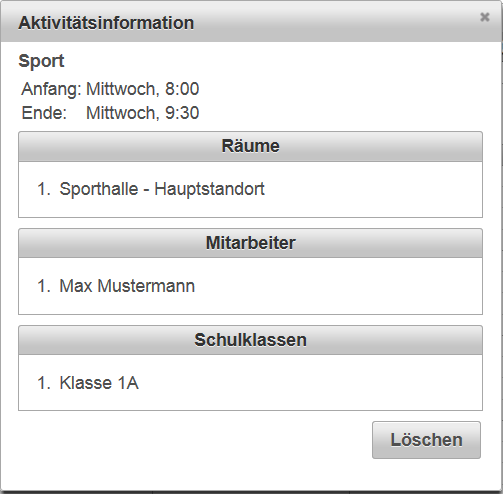
\includegraphics[width=0.5\textwidth]{images/activityInfo.png}
\end{figure}

\subsubsection{Löschen einer Aktivität}
\begin{enumerate}
\item Führen Sie einen Linksklick auf die zu löschende Aktivität aus.
\item Klicken Sie im nun geöffneten Dialog auf den "`Löschen"'-Button. \medskip\\
	\begin{minipage}[t]{\linewidth}
            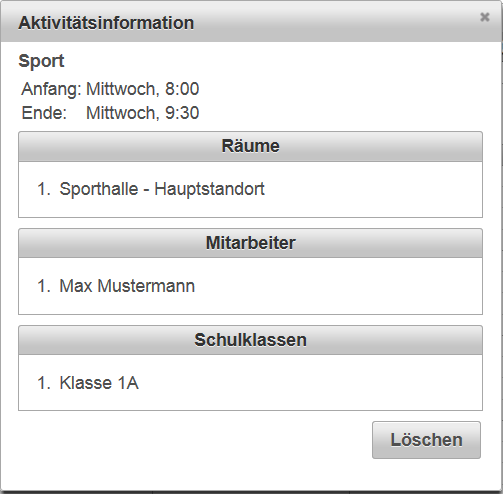
\includegraphics[width=.5\linewidth]{images/activityInfo.png}
    \end{minipage} 
    \medskip\\
    Die Aktivität wurde gelöscht. Sie können diese Aktion natürlich auch rückgängig machen.
\end{enumerate}

\subsubsection{Drag \& Drop}
Sie können im Stundenplan Drag \& Drop nutzen um Aktivitäten an andere Tage oder Uhrzeiten zu verschieben. Klicken Sie dazu die zu verschiebende Aktivität an und halten die linke Maustaste gedrückt, ziehen Sie die Aktivität zum gewünschten Zeitraum und lassen Sie die linke Maustaste los.\\
Des weiteren kann die Dauer einer Aktivität auf ähnliche Art und Weise verändern. Zeigen Sie mit der Maus auf den unteren Rand einer Aktivität, so dass ein nach oben und unten zeigender Pfeil erscheint, halten Sie nun die linke Maustaste gedrückt und ziehen sie das Ende der Aktivität auf den gewünschten Endzeitpunkt. Lassen Sie die Maustaste los und die Aktivität wird aktualisiert. \\

\subsubsection{Überschneidungen}
Beim Hinzufügen von Aktivitäten und dem Verändern via Drag \& Drop kann es natürlich immer zu Überschneidungen mit anderen Aktivitäten von einem der Teilnehmer kommen. Ist dies der Fall, erhalten Sie eine entsprechende Fehlernachricht und die Aktivität wird auf Ihren ursprünglichen Zustand zurückgesetzt.

\subsubsection{Überschreitung des Wochenstundenkontingents}
Sollte das Hinzufügen einer Aktivität zu einer Überschreitung des Wochenstundenkontingents bei einer der teilnehmenden Personen des Personals führen, wird das Hinzufügen der Aktivität nicht unterbunden. Sie erhalten jedoch eine Warnmeldung: 

\begin{figure}[H]
\centering
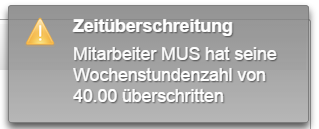
\includegraphics[width=0.4\textwidth]{images/warning.png}
\end{figure}


\section{Fehler und Fehlerbehandlung}
\renewcommand{\arraystretch}{1.5}
\begin{tabularx}{\textwidth}{|p{5cm}|X|}
\hline
\textbf{Fehler} & \textbf{Fehlerbeschreibung und mögliche Fehlerbehandlung}\\\hline
Backup-Wiederherstellung fehlgeschlagen & Dieser Fehler tritt auf, wenn es nicht möglich war, den im Backup enthaltenen Datenbankzustand wiederherzustellen. Versuchen Sie ggf. noch einmal das Backup wiederherzustellen, schlägt es weiterhin fehl, ist das Backup ggf. beschädigt.\\\hline
Datenbankfehler & Dieser Fehler tritt auf, wenn es ein internes Problem mit der Kommunikation mit der Datenbank gibt. Wenn der Fehler mehr als einmal auftritt, versuchen Sie einen Neustart der Software.\\\hline
Fehler beim Laden der Einstellungen & Dieser Fehler tritt auf, wenn die Datei \textit{timetable.properties} ungültige Einträge besitzt. Falls Sie manuell Änderungen an der Datei vorgenommen haben, machen Sie diese rückgängig. Ansonsten können Sie die Datei auch löschen, beim nächsten Systemstart werden dann die Standardeinstellungen wiederhergestellt. Beachten Sie dabei, dass dann Aktivitäten außerhalb der standardmäßigen Start- und Endzeiten eines Wochentags liegen könnten und lediglich nicht angezeigt werden. Die Aktivitäten werde nicht automatisch gelöscht.\\\hline
System nicht vollständig wiederhergestellt & Dieser Fehler tritt bei der Wiederherstellung auf, wenn die Datei \textit{timetable.properties} aus dem Backup nicht in das Arbeitsverzeichnis kopiert werden konnte. Kopieren Sie die Datei manuell in das Arbeitverzeichnis.\\\hline
Ungültige Datei & Dieser Fehler tritt beim Wiederherstellen eines Backups auf, wenn eine ZIP-Datei zur Wiederherstellung gewählt wurde, welche kein Backup repräsentiert.\\\hline
\end{tabularx}\\

Neben den oben aufgeführten Fehlermeldungen existieren einige weitere Fehlermeldungen im System, bei diesen ist der Grund für den Fehler und damit die Behandlung des Fehlers jedoch offensichtlich.

\end{document}
